\section{Finite laws and geometric conventions}\label{sec:conventions}

We fix the finite conditioning, planar duality, and boundary-incidence
conventions used throughout the proof. The distinction between a path
in a quotient graph and a path made of physical open edges is essential:
the comparison inequalities first concern the former, while the
crossing estimates for explored domains must eventually control the latter.

\subsection{Odds, identifications, and conditional laws}

For a finite graph $G=(V,E)$ with positive edge odds $v_e$, write
\begin{equation}\label{eq:odds-partition}
 Z_G(q,\mathbf v)=\sum_{A\subseteq E}q^{k(A)}\prod_{e\in A}v_e.
\end{equation}
Parallel edges and loops are allowed. A boundary partition $\xi$ means
the quotient graph obtained by identifying vertices in each class.
Identifications are not sampled edges. A loop contributes a factor
$1+v_e$ to the partition function and does not affect other edges.
In the square medium all ordinary odds are $v_e=d$.

\begin{lemma}[Finite conditioning and bounded local changes]
\label{lem:finite-conditioning}
Conditioning on any set of edge states gives the random-cluster law on
the remaining graph with the identifications induced by the open
conditioned edges and the original partition. Conditional on all other
edge states, an edge of odds $v$ has opening probability either
$v/(1+v)$ or $v/(q+v)$, according as its endpoints are already connected
or not. Changing a bounded number of edge states or pairwise vertex identifications
therefore has bounded positive weight cost when the affected odds stay
in a fixed compact subset of $(0,\infty)$.
\end{lemma}
\begin{proof}
Contract the open conditioned edges and delete the closed ones.
Components that no longer contain an unconditioned vertex contribute
a fixed power of $q$. All other components are counted in the quotient
graph, giving \eqref{eq:odds-partition}. Adding an edge to a fixed
state either leaves its component count unchanged or reduces it by
one, so its opening-to-closing odds are $v$ or $v/q$.
A single identification of two vertices similarly multiplies a state's weight
by $1$ or $q^{-1}$. Products of a fixed number of such factors, including
the normalizing constants, give the last assertion.
\end{proof}

The same statement applies to a stopped exploration. A leaf of its
decision tree specifies exactly the edge states it has revealed;
no additional event in the uninspected region may be conditioned on
when invoking Lemma~\ref{lem:finite-conditioning}.

\begin{definition}[Network and actual connections]
\label{def:actual-network}
A \emph{network connection} is an open connection in the graph after
the prescribed vertex identifications. An \emph{actual connection}
uses open physical edges and does not jump between distinct vertices
in a boundary class. A measured actual path may subsequently be
contracted to a terminal when its opposite side remains uninspected.
\end{definition}

With only two disjoint separately wired electrode sets, their network
connection is equivalent to an actual path between the sets. Extra
boundary wires can invalidate this equivalence. We will explicitly
remove such shortcuts whenever converting a network test to an actual
path assertion.

\subsection{Tiles, caps, and Euler's identity}

We use checkerboard square tiles whose sides make angle $\pi/4$ with
the primal lattice axes. A tile has one primal diagonal, one dual
diagonal, and a port at each side midpoint. Opening the primal diagonal
pairs the ports around the dual corners; closing it opens the dual
diagonal and pairs the ports around the primal corners. Corners of a
fixed color on one side of a switch strand are connected by actual
edges on that side. The tile drawing only records the same edge state,
not a different random model. Figure~\ref{fig:local-switch} records
the two local states.

\begin{figure}[tbp]
\centering
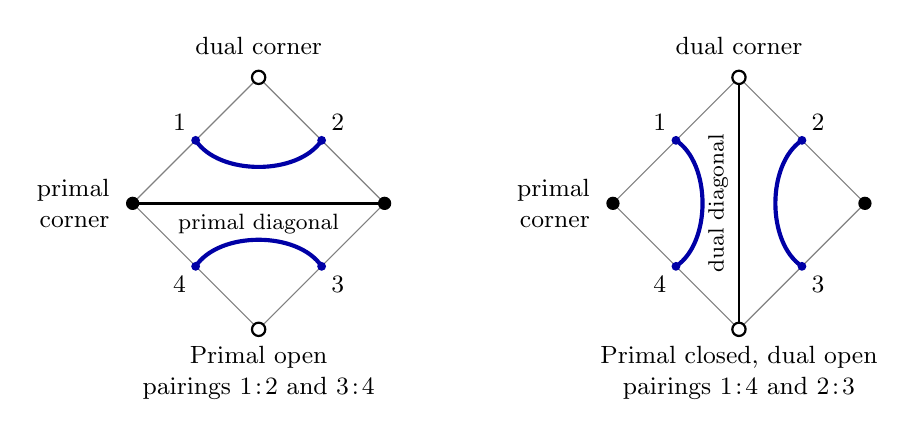
\begin{tikzpicture}[x=1cm,y=1cm,font=\small,line cap=round,line join=round]
  \foreach \shift in {0,6.1} {
    \begin{scope}[xshift=\shift cm]
      \draw[gray] (-1.6,0) -- (0,1.6) -- (1.6,0) -- (0,-1.6) -- cycle;
      \node[above] at (0,1.77) {dual corner};
      \node[left,align=right] at (-1.77,0) {primal\\corner};
      \node[above left] at (-.8,.8) {$1$};
      \node[above right] at (.8,.8) {$2$};
      \node[below right] at (.8,-.8) {$3$};
      \node[below left] at (-.8,-.8) {$4$};
    \end{scope}
  }
  \draw[line width=1pt] (-1.6,0) -- (1.6,0);
  \node[below,font=\footnotesize] at (0,-.015) {primal diagonal};
  \draw[blue!65!black,line width=1.5pt]
    (-.8,.8) .. controls (-.5,.35) and (.5,.35) .. (.8,.8);
  \draw[blue!65!black,line width=1.5pt]
    (-.8,-.8) .. controls (-.5,-.35) and (.5,-.35) .. (.8,-.8);
  \begin{scope}[xshift=6.1cm]
    \draw[line width=1pt] (0,-1.6) -- (0,1.6);
    \node[rotate=90,above,font=\footnotesize] at (-.015,0) {dual diagonal};
    \draw[blue!65!black,line width=1.5pt]
      (-.8,.8) .. controls (-.35,.5) and (-.35,-.5) .. (-.8,-.8);
    \draw[blue!65!black,line width=1.5pt]
      (.8,.8) .. controls (.35,.5) and (.35,-.5) .. (.8,-.8);
  \end{scope}
  \foreach \shift in {0,6.1} {
    \begin{scope}[xshift=\shift cm]
      \fill (-1.6,0) circle (2.4pt);
      \fill (1.6,0) circle (2.4pt);
      \draw[fill=white,line width=.8pt] (0,1.6) circle (2.4pt);
      \draw[fill=white,line width=.8pt] (0,-1.6) circle (2.4pt);
      \foreach \x/\y in {-.8/.8,.8/.8,.8/-.8,-.8/-.8}
        \fill[blue!65!black] (\x,\y) circle (1.6pt);
    \end{scope}
  }
  \node[align=center] at (0,-2.15)
    {Primal open\\pairings $1\!:\!2$ and $3\!:\!4$};
  \node[align=center] at (6.1,-2.15)
    {Primal closed, dual open\\pairings $1\!:\!4$ and $2\!:\!3$};
\end{tikzpicture}
\caption{The two local switch states, with ports numbered clockwise. Black dots are primal corners and white dots are dual corners. The black diagonal is the open physical bond; the complementary diagonal is omitted. Blue curves are medial strands: an open primal bond pairs ports around the dual corners, while an open dual bond pairs ports around the primal corners. The switch drawing records the same FK edge state and introduces no additional randomness.}
\label{fig:local-switch}
\end{figure}


A \emph{wall} cuts tile-to-tile port contractions and keeps its two
banks separate. At a boundary interval designated primal-wired or
dual-wired, local caps pair the intervening ports between successive
visits of the designated vertex color. Boundary-condition changes
leave unmatched ports. A positive
completion pairs the unmatched ports by the specified planar cap
trees, so that the switch diagram is a finite collection of loops.

\begin{lemma}[Positive loop law]\label{lem:loop-law}
For any fixed planar cap completion, the weight of a switch state in
the homogeneous medium is proportional to $d^{\ell}$, where $\ell$
is its number of completed loops and $d=\sqrt q$.
The proportionality factor is independent of the switch state.
Changing a bounded number of loose-port pairings has bounded positive
weight cost for every fixed $d>0$.
\end{lemma}
\begin{proof}
Thicken the open primal graph together with the fixed boundary cap
trees on the sphere. If a planar ribbon graph has $V'$ vertices,
$E'$ edges, and $k'$ components, then its regular neighborhood has
Euler characteristic $V'-E'$ and also $2k'-\ell$, because every
component has genus zero. Thus $\ell=2k'+E'-V'$.
The cap trees change the expression only by a constant depending on
the fixed completion, and their contractions make $k'=k_\xi(A)$.
Consequently
\[
 \ell=2k_\xi(A)+|A|+c_\xi,
 \qquad
 d^\ell=d^{c_\xi}q^{k_\xi(A)}d^{|A|}.
\]
This is the odds form of the FK weight. A change of one pairing can
merge or split only a bounded number of loops. Its weight ratio is
therefore bounded above and below by fixed powers of $d$; normalization
preserves a bounded two-sided comparison.
\end{proof}

On a torus the same thickening has total genus at most one, so the
formula gains $-2g$ with $g\in\{0,1\}$. The loop/FK discrepancy is
then a bounded genus factor. This fact will be used only in the
explicit torus-to-plane comparison of Section~\ref{sec:physical}.

\begin{lemma}[Finite planar duality]\label{lem:finite-duality}
Complementary dual-open edges have odds $q/v_e$. In particular the
homogeneous square medium with odds $d=\sqrt q$ is self-dual.
Complementary boundary caps are understood on the same cut surface.
\end{lemma}
\begin{proof}
For a connected plane graph on the sphere, the dual subgraph on
$E\setminus A$ has as many components as the faces of the primal
subgraph. Euler's identity gives
$k^*(E\setminus A)=|A|-|V|+k(A)+1$.
Multiplying out $q^{k^*(E\setminus A)}
\prod_{e\notin A}(q/v_e)$ shows that its ratio to
$q^{k(A)}\prod_{e\in A}v_e$ is constant in $A$.
Fixed cap trees can be included before applying this identity and
then contracted; their complementary dual incidences give the stated
boundary convention. Disconnected ambient graphs are handled
componentwise or by adding fixed exterior trees.
\end{proof}

\subsection{Cut surfaces and the order of limits}

A tiled disk has an injectively embedded open interior. Boundary
incidences are counted on the disk itself: the two banks of a slit or
the two fans at a pinched vertex are distinct even if their planar
images agree. The specific half-tile and triangular boundary pieces
used below carry the ordinary bonds specified in their construction.
Their conditional law, including any required resampling of cut cells,
is justified when each construction is introduced. A cut does not
identify coincident banks.

A cap partition is \emph{planar} if its classes can be connected by
noncrossing arcs in the designated exterior. A pair of end caps is
\emph{separate} when neither cap joins the two ends. A joint planar
end partition may join them, but is still supported only on those
end intervals. Statements allowing a bounded number of through hubs
will explicitly require that, after removing all classes meeting
those hubs, the residual caps remain separately planar. No assertion
about arbitrary crossing partitions is implicit.

An extremal search starts from a specified exterior complementary face.
It queries an edge only from a reached face and enters the opposite face
only when the intervening edge of the tested color is closed. After
exploring the complete reached component, it selects the appropriate
simple frontier from the measured open edges. On success this frontier
is a blocker whose opposite side remains uninspected. Boundary access
arcs used to define the search do not identify vertices or add physical
edges. Prefixes and stopped leaves retain the cyclic order of the
boundary incidences.

Raw arcs, passages, and nests are counted before the ports at any
wall are paired. This avoids changing a local count by a remote cap
identification. All comparisons concern positive finite laws unless
a signed spin or charge expansion is explicitly specified.

Throughout the paper $q$ is fixed. Constants may depend on $q$,
fixed charges, and fixed shape and buffer parameters. In a geometric
argument the finite inventory of shapes, clearances, gaps, and auxiliary
ratios is chosen before the mesh is sent to zero. A large-circle
transfer limit is taken with the finite insertion diagram fixed;
later mesh or insertion limits follow it. When a relative error is
needed rather than a bounded multiplicative comparison, it is stated
as such. These orders will also be recorded at the points where
several limits interact.
